\setcounter{section}{35}
\setcounter{ex}{0}
\section{Viết PTĐT}
\subsection{Kiến thức cần nhớ}
\begin{khung}
	\subsubsection{Véc-tơ chỉ phương của đường thẳng}
	\begin{itemize}
\begin{multicols}{2}
\item Cho đường thẳng $\Delta$, véc-tơ $\vec{u}\ne\vec{0}$ gọi là véc-tơ chỉ phương của đường thẳng $\Delta$ nếu giá của nó song song hoặc trùng với $\Delta$.

\columnbreak

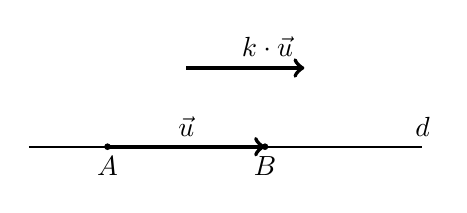
\begin{tikzpicture}
	\draw[thick] (0,0) -- (5,0) node [above]{$d$};
	\draw[line width=1.5pt, ->] (1,0)--(3,0);
	\fill (1,0) node [below] {$A$}circle (1.2pt);
	\fill (3,0) node [below] {$B$}circle (1.2pt);
	\draw (2,0) node [above] {$\vec{u}$};
	\draw[line width=1.5pt, ->] (2,1)--(3.5,1) node [above left] {$k\cdot\vec{u}$};
\end{tikzpicture}
\end{multicols}
\item  Cho đường thẳng $\Delta$ đi qua $M(x_0;y_0;z_0)$ và có véc-tơ chỉ phương là $\vec{u}=(a;b;c)$.
\item Nếu $\vec{u}$ là véc-tơ chỉ phương của $\Delta$ thì $k\cdot\vec{u}$ $(k\ne 0)$ cũng là véc-tơ chỉ phương của $\Delta$.
\item Nếu đường thẳng $\Delta$ đi qua hai điểm $A$, $B$ thì $\overrightarrow{AB}$ là một véc-tơ chỉ phương.
	\end{itemize}
	\subsubsection{Viết PTĐT}
	\begin{itemize}
\item Biết đường thẳng $d$ đi qua điểm $M_0(a_1;a_2;a_3)$ và có véc-tơ chỉ phương $\vec{a}=(a_1;a_2;a_3)$, $(\vec{a}\neq \vec{0})$, khi đó PTTS của $d$ là $\heva{x=x_0+a_1t \\y= y_0 + a_2t \\ z=z_0+a_3t}$, $(t\in\mathbb{R})$
\item Nếu $a_1$, $a_2$, $a_3$ đều khác không. PTĐT $d$ viết dưới dạng chính tắc như sau
\[\dfrac{x-x_0}{a_1}=\dfrac{y-y_0}{a_2}=\dfrac{z-z_0}{a_3}\]
	\end{itemize}
\end{khung}
\subsection{Bài tập mẫu}
\Opensolutionfile{ans}[ans/ANS-DANG-36]
\begin{khung}
	\begin{vd}[Đề minh họa BGD 2022-2023]%[Trương Đăng Khoa]%[1D2Y2-1]
Trong KG $Oxyz$, cho hai điểm $M(1;-1;-1)$ và $N(5;5;1)$. Đường thẳng $MN$ có phương trình là
		\choice
		{$\heva{&x=5+2t\\&y=5+3t\\&z=-1+t}$}	
		{$\heva{&x=5+t\\&y=5+2t\\&z=1+3t}$}
		{\True $\heva{&x=1+2t\\&y=-1+3t\\&z=-1+t}$}	
		{$\heva{&x=1+2t\\&y=-1+t\\&z=-1+3t}$}
		\loigiai{
Đường thẳng $MN$ đi qua $M(1;-1;-1)$ và nhận $\vv{MN}=2(2;3;1)$ làm véc-tơ chỉ phương nên có phương trình $\heva{&x=1+2t\\&y=-1+3t\\&z=-1+t.}$
		}
	\end{vd}
\end{khung}
\subsection{Bài tập tương tự và phát triển}
\begin{ex}%[Trương Đăng Khoa]%[2H3Y3-2]
	Trong không gian $O x y z$, cho đường thẳng $\Delta$ đi qua điểm $M(2;0;-1)$ và có một véc-tơ chỉ phương $\vec{a}=(4;-6;2)$. PTTS của $\Delta$ là 
	\choice 
	{\True $\heva{&x=2+2t\\&y=-3t\\&z=-1+t}$}
	{$\heva{&x=4+2t\\&y=-6\\&z=2+t}$}
	{$\heva{&x=-2+2t\\&y=3t\\&z=1+t}$}
	{$\heva{&x=-2+4t\\&y=6t\\&z=1+2t}$}
					\loigiai 
					{
Ta có $\vec{a}=(4;-6;2)=2(2;-3;1)$.\\
Do đó đường thẳng $\Delta$ có một véc-tơ chỉ phương là $\vec{u}=(2;-3;1)$.\\
Vậy PTTS của $\Delta$ đi qua $M(2;0;-1)$ và có một véc-tơ chỉ phương là $\vec{u}=(2;-3;1)$ là $\heva{&x=2+2t\\&y=-3t\\&z=-1+t}$.\\
					}
\end{ex}

\begin{ex}%[Trương Đăng Khoa]%[2H3B3-2]
	Trong không gian với hệ tọa độ $O x y z$, cho hai điềm $A(1;1;2)$, $B(2;-1;3)$. Viết PTĐT $AB$.
	\choice 
	{\True $\dfrac{x-1}{1}=\dfrac{y-1}{-2}=\dfrac{z-2}{1}$}
	{$\dfrac{x+2}{1}=\dfrac{y-1}{-2}=\dfrac{z+3}{1}$}
	{$\dfrac{x+1}{1}=\dfrac{y+1}{2}=\dfrac{z+2}{1}$}
	{$\dfrac{x+2}{1}=\dfrac{y-1}{2}=\dfrac{z+3}{1}$}
	\loigiai 
	{
Ta có $\vv{AB}=(1;-2;1)$.\\
Đường thẳng $AB$ đi qua điểm $A(1;1;2)$ và nhận véc-tơ $\vv{AB}=(1;-2;1)$ làm véc-tơ chỉ phương.\\
Vậy phương trình của $AB$ là $\dfrac{x-1}{1}=\dfrac{y-1}{-2}=\dfrac{z-2}{1}$.
	}
\end{ex}

\begin{ex}%[Trương Đăng Khoa]%[2H3B3-2]
Trong không gian $O x y z$, PTĐT đi qua 2 điểm $M(2;-1;1)$ và $N(0;1;3)$ là 
\choice 
{$\heva{&x=2\\&y=-1+t\\&z=1+3t}$}
{$\heva{&x=2+t\\&y=1-t\\&z=-1-t}$}
{$\heva{&x=2+t\\&y=-1\\&z=1+2t}$}
{\True $\heva{&x=2+t\\&y=-1-t\\&z=1-t}$}
\loigiai
{
$\vv{M N}=(-2;2;2)$.
$\Rightarrow$ $\vec{u}=-\dfrac{1}{2}\vv{MN}=(1;-1;-1)$ là một véc-tơ chỉ phương của đường thẳng $MN$. Do đó PTĐT $MN$ là $\heva{&x=2+t\\&y=-1-t\\&z=1-t}$, ($t\in\mathbb{R}$).
}
\end{ex}

\begin{ex}%[Trương Đăng Khoa]%[2H3B3-2]
	Trong không gian $O x y z$, cho điểm $M(3;-2;2)$ và mặt phẳng $(P): x+3y-2z=0$. Đường thẳng $\Delta$ đi qua $M$ và vuông góc với $(P)$ có PTTS là 
	\choice 
	{$\heva{&x=3+t\\&y=-2+3t\\&z=-2-2t}$}
	{\True $\heva{&x=3+t\\&y=-2+3t\\&z=2-2t}$}
	{$\heva{&x=3-t\\&y=-2-3t\\&z=2-2t}$}
	{$\heva{&x=3-t\\&y=-2-3t\\&z=-2+2t}$}
					\loigiai 
					{
Mặt phẳng $(P)\colon x+3y-2z=0$ có một véc-tơ pháp tuyến $\vec{n}=(1;3;-2)$.\\
Đường thẳng $\Delta$ vuông góc với $(P)$ nên có véc-tơ chỉ phương $\vec{u}=\vec{n}=(1;3;-2)$.\\
PTĐT $\Delta$ là $\heva{&x=3+t\\&y=-2+3t\\&z=2-2t.}$	
					}
\end{ex}

\begin{ex}%[Trương Đăng Khoa]%[2H3B3-2]
	Trong không gian với hệ tọa độ $O x y z$, cho hai điểm $A(1;2;-3)$, $B(-2;3;1)$ đường thẳng đi qua $A(1;2;-3)$ và song song với $OB$ có phương trình là 
	\choice 
	{$\heva{&x=-2+t\\&y=3+2t\\&z=1-3t}$}
	{\True $\heva{&x=1-2t\\&y=2+3t\\&z=-3+t}$}
	{$\heva{&x=1-4t\\&y=2-6t\\&z=-3+2t}$}
	{$\heva{&x=1-2t\\&y=2+3t\\&z=-3-t}$}
					\loigiai 
					{
	Ta có $\vv{OB}=(-2;3;1)$ là véc-tơ chỉ phương của đường thẳng cần tìm.\\
	PTĐT qua $A(1;2;-3)$ và song song với $OB$ là $\heva{&x=1-2t\\&y=2+3t\\&z=-3+t.}$
					}
\end{ex}

\begin{ex}%[Trương Đăng Khoa]%[2H3Y3-2]
Trong không gian $O x y z$, PTTS của đường thẳng $d$ đi qua điểm $M(1;2;3)$ và có véc-tơ chỉ phương $\vec{a}=(1;-4;-5)$ là 
\choice 
{$\heva{&x=1+t\\&y=-4+2t\\&z=-5+3t}$}
{$\dfrac{x-1}{1}=\dfrac{y+4}{2}=\dfrac{z+5}{3}$}
{$\heva{&x=1-t\\&y=2+4t\\&z=3+5t}$\True}
{$\dfrac{x-1}{1}=\dfrac{y-2}{-4}=\dfrac{z-3}{-5}$}
\loigiai{
Vì $d$ có véc-tơ chỉ phương $\vec{a}=(1;-4;-5)$, suy ra $d$ cũng có một véc-tơ chỉ phương khác nữa là $\vec{b}=(-1;4;5)$. PTTS của đường thẳng $d$ đi qua điểm $M(1;2;3)$ và có véc-tơ chỉ phương $\vec{b}=(-1;4;5)$ là $\heva{&x=1-t\\&y=2+4 t\\&z=3+5t.}$
}
\end{ex}

\begin{ex}%[Trương Đăng Khoa]%[2H3Y3-2]
	Cho đường thẳng $d$ có PTTS $\heva{&x=3+2t\\&y=1-4t\\&z=5+7t}$, ($t\in\mathbb{R}$). Tìm phương trình chính tắc của đường thẳng $d$.
		\choice 
		{$d\colon2(x-3)-4(y-1)+7(z-5)=0$}
		{$d\colon\dfrac{x-2}{3}=\dfrac{y+4}{1}=\dfrac{z-7}{5}$}
		{$d\colon3(x-2)+y+4+5(z-7)=0$}
		{$d\colon\dfrac{x-3}{2}=\dfrac{y-1}{-4}=\dfrac{z-5}{7}$\True}
		\loigiai 
		{
Từ PTTS của đường thẳng $d$ ta có $d$ đi qua điểm $A(3;1;5)$ và có một véc-tơ chỉ phương là $\vec{u}=(2;-4;7)$. Do đó $d$ có phương trình chính tắc là $\dfrac{x-3}{2}=\dfrac{y-1}{-4}=\dfrac{z-5}{7}$.
		}
	\end{ex}

\begin{ex}%[Trương Đăng Khoa]%[2H3Y3-2]
	Trong không gian $O x y z$, đường thẳng chứa trục $O y$ có PTTS là 
	\choice 
	{$\heva{&x=0\\&y=1\\&z=t}$}
		{\True $\heva{&x=0\\&y=t\\&z=0}$}
			{$\heva{&x=t\\&y=0\\&z=0}$}
				{$\heva{&x=0\\&y=0\\&z=t}$}
					\loigiai 
					{
		Trục $O y$ qua $O(0;0;0)$ và có véc-tơ chỉ phương $\vec{j}=(0;1;0)$ nên có phương trình $\heva{&x=0\\&y=t\\&z=0.}$
					}
\end{ex}

\begin{ex}%[Trương Đăng Khoa]%[2H3Y3-2]
	Trong không gian với hệ tọa độ $O x y z$, cho đường thẳng $d\colon\heva{&x=2-t\\&y=1+t\\ &z=t}$. Phương trình nào sau đây là phương trình chính tắc của $d$?
		\choice 
		{$\dfrac{x+2}{1}=\dfrac{y}{-1}=\dfrac{z-3}{1}$}
		{$x-2=y=z+3$}
		{\True $\dfrac{x-2}{-1}=\dfrac{y-1}{1}=\dfrac{z}{1}$}
		{$\dfrac{x-2}{-1}=\dfrac{y}{1}=\dfrac{z+3}{-1}$}
		\loigiai 
		{
Đường thẳng $d$ có véc-tơ chỉ phương $\vec{u}=(-1;1;1)$ và đi qua điểm $M(2;1;0)$. Do đó phương trình chính tắc của $d$ là $\dfrac{x-2}{-1}=\dfrac{y-1}{1}=\dfrac{z}{1}$.		
		}
\end{ex}

\begin{ex}%[Trương Đăng Khoa]%[2H3B3-2]
	Trong không gian $O x y z$, viết phương trình chính tắc đường thẳng $d$ đi qua điểm $A(1;2;3)$ và vuông góc với mặt phẳng $(P)\colon 2x+2y+z+2023=0$.
	\choice 
	{$\dfrac{x+1}{2}=\dfrac{y+2}{2}=\dfrac{z+3}{1}$}
	{\True $\dfrac{x-1}{2}=\dfrac{y-2}{2}=\dfrac{z-3}{1}$}
	{$\dfrac{x-2}{1}=\dfrac{y-2}{2}=\dfrac{z-1}{3}$}
	{$\dfrac{x+2}{1}=\dfrac{y+2}{2}=\dfrac{z+1}{3}$}
	\loigiai 
	{
Đường thẳng $d$ có véc-tơ chỉ phương là véc-tơ pháp tuyến của mặt phẳng $(P)$ là $\vec{u}=(2;2;1)$.\\
Do đó phương phương trình chính tắc đường thẳng $d$ là $\dfrac{x-1}{2}=\dfrac{y-2}{2}=\dfrac{z-3}{1}$.
	}
\end{ex}

\begin{ex}%[Trương Đăng Khoa]%[2H3Y3-2]
	Trong không gian với hệ tọa độ $O x y z$, cho đường thẳng $\Delta$ có phương trình chính tắc là $\dfrac{x+2}{1}=\dfrac{y-1}{-1}=\dfrac{z}{2}$. Hỏi phương trình nào sau đây là PTTS của $\Delta$?
	\choice 
	{$\heva{&x=-2+t\\&y=1-t\\&z=t}$}
		{$\heva{&x=2+t\\&y=-1-t\\&z=2t}$}
			{\True $\heva{&x=-2+t\\&y=1-t\\&z=2t}$}
				{$\heva{&x=-2-t\\&y=1-t\\&z=-2t}$}
					\loigiai 
					{
$(\Delta)\colon \dfrac{x+2}{1}=\dfrac{y-1}{-1}=\dfrac{z}{2}$.\\
Suy ra $(\Delta)$ đi qua điểm $A(-2;1;0)$ và có véc-tơ chỉ phương $\vec{u}=(1;-1;2)$.\\
Vậy PTTS $(\Delta)\colon \heva{ &x=-2+t\\&y=1-t\\&z=2t.}$
					}
\end{ex}

\begin{ex}%[Trương Đăng Khoa]%[2H3B3-2]
	Trong không gian $O x y z$, cho điểm $M(1;0;-1)$ và đường thẳng $d\colon\dfrac{x-2}{4}=\dfrac{y-1}{-5}=\dfrac{z-3}{2}$. Đường thẳng $\Delta$ đi qua $M$ và song song với $d$ có PTTS là 
	\choice 
	{$\heva{&x=1-4t\\&y=5t\\&z=-1+2t}$}
		{$\heva{&x=1+2t\\&y=t\\&z=-1+3t}$}
			{\True $\heva{&x=1+4t\\&y=-5t\\&z=-1+2t}$}
				{$\heva{&x=-1-4t\\&y=5t\\&z=-1-2t}$}
					\loigiai 
					{
$d\colon\dfrac{x-2}{4}=\dfrac{y-1}{-5}=\dfrac{z-3}{2}$ có một véc-tơ chỉ phương là $\vec{u}(4;-5;2)$.\\
Đường thẳng $\Delta$ song song với $d$ nên có véc-tơ chỉ phương là $\vec{u}(4;-5;2)$.\\
PTĐT $\Delta$ là $\heva{&x=1+4t\\&y=-5t\\&z=-1+2t.}$
					}
				\end{ex}
			
\begin{ex}%[Trương Đăng Khoa]%[2H3Y3-2]
	Trong không gian $O x y z$, phương trình chính tắc của đường thẳng $(d)\colon\heva{&x=1-2t\\&y=3t\\&z=2+t}$ là 
		\choice 
		{$\dfrac{x+1}{-2}=\dfrac{y}{3}=\dfrac{z+2}{1}$}
		{$\dfrac{x-1}{2}=\dfrac{y}{3}=\dfrac{z+2}{2}$}
		{$\dfrac{x+1}{1}=\dfrac{y}{3}=\dfrac{z-2}{2}$}
		{\True $\dfrac{x-1}{-2}=\dfrac{y}{3}=\dfrac{z-2}{1}$}
		\loigiai 
		{
	Ta có đường thẳng $(d)$ đi qua điểm $A(1;0;2)$ và có một véc-tơ chỉ phương là $\vec{u}=(-2;3;1)$ nên có phương trình chính tắc là $\dfrac{x-1}{-2}=\dfrac{y}{3}=\dfrac{z-2}{1}$.
		}
	\end{ex}

\begin{ex}%[Trương Đăng Khoa]%[2H3Y3-2]
	Trong không gian $O x y z$, cho hai điểm $M(2;1;2)$ và $N(4;3;-2)$. Đường thẳng $MN$ có PTTS là 
	\choice 
	{$\heva{&x=4+2t\\&y=3+2t.\\&z=2-4t}$}
		{$\heva{&x=2+t\\&y=1+t\\&z=2+2t}$}
			{$\heva{&x=-1+t\\&y=-2+t\\&z=11-2t}$}
				{\True $\heva{&x=-3-t\\&y=-4-t\\&z=12+2t}$}
					\loigiai 
					{
	Ta có: $\vec{MN}=(2;2;-4)$ nên chọn $\vec{u}=(1;1;-2)$ là véc-tơ chỉ phương của $MN$.\\
	Đường thẳng $MN$ có véc-tơ chì phương là $\vec{u}=(1;1;-2)$ và đi qua điểm $M(2;1;2)$ nên có PTTS là $\heva{&x=-3-t\\&y=-4-t\\&z=12+2t.}$
					}
				\end{ex}
	
\begin{ex}%[Trương Đăng Khoa]%[2H3Y3-2]
	Trong không gian với hệ tọa độ $O x y z$, cho đường thẳng $\Delta$ đi qua điểm $M(2;0;-1)$ và có véc-tơ chì phương $\vec{a}=(4;-6;2)$. PTTS của $\Delta$ là 
	\choice 
	{\True $\heva{&x=2+2t\\&y=-3t\\&z=-1+t}$}
		{$\heva{&x=-2+2t\\&y=-3t\\&z=1+t}$}
			{$\heva{&x=4+2t\\&y=-6-3t.\\&z=2+t}$}
				{$\heva{&x=-2+4t\\&y=-6t\\&z=1+2t}$}
					\loigiai 
					{
Vì $\Delta$ có véc-tơ chỉ phương $\vec{a}=(4;-6;2)$ nên $\Delta$ cũng nhận véc-tơ $\dfrac{1}{2}\vec{a}=(2;-3;1)$ làm véc-tơ chỉ phương. Do đó PTTS của $\Delta$ là $\heva{&x=2+2t\\&y=-3t\\&z=-1+t.}$
					}
\end{ex}

\begin{ex}%[Trương Đăng Khoa]%[2H3B3-2]
	Trong không gian với hệ trục tọa độ $O x y z$, cho mặt phẳng $(P)\colon 3x-y+6z-18=0$. Đường thẳng $d$ đi qua $A(2;1;0)$ và vuông góc với mặt phẳng $(P)$ có dạng là 
	\choice 
	{$d\colon\dfrac{x-2}{-3}=\dfrac{y-1}{1}=\dfrac{z-3}{-6}$}
	{\True $d\colon\dfrac{x-2}{3}=\dfrac{y-1}{-1}=\dfrac{z}{6}$}
	{$d\colon\dfrac{x-3}{2}=\dfrac{y+1}{1}=\dfrac{z-2}{3}$}
	{$d\colon\dfrac{x-2}{2}=\dfrac{y-1}{1}=\dfrac{z}{5}$}
	\loigiai 
	{
Mặt phẳng $(P)\colon 3x-y+6z-18=0$ có $\vec{n}=(3;-1;6)$ là véc-tơ pháp tuyến.\\
Ta có $d$ vuông góc với mặt phẳng $(P)$ nên $d$ có $\vec{u}_d=(3;-1;6)$ là véc-tơ chỉ phương $d$ đi qua $A(2;1;0)$ và có $\vec{u}_d=(3;-1;6)$ là véc-tơ chỉ phương nên $d$ có phương trình là $d\colon \dfrac{x-2}{3}=\dfrac{y-1}{-1}=\dfrac{z}{6}$.
	}
\end{ex}

\begin{ex}%[Trương Đăng Khoa]%[2H3B3-2]
	Trong không gian $O x y z$, đường thẳng đi qua điểm $A(1;4;-7)$ và vuông góc với mặt phẳng $x+2y-2z-3=0$ có phương trình là 
	\choice 
	{$\dfrac{x-1}{1}=\dfrac{y-4}{-2}=\dfrac{z+7}{-2}$}
	{\True $\dfrac{x-1}{1}=\dfrac{y-4}{2}=\dfrac{z+7}{-2}$}
	{$\dfrac{x-1}{1}=\dfrac{y-4}{2}=\dfrac{z-7}{-2}$}
	{$\dfrac{x+1}{1}=\dfrac{y+4}{4}=\dfrac{z-7}{-7}$}
	\loigiai 
	{
Đường thẳng đi qua điểm $A(1;4;-7)$ và vuông góc với mặt phẳng $x+2y-2z-3=0$ nên có một véc-tơ chỉ phương $\vec{u}=(1;2;-2)$ có phương trình là $\dfrac{x-1}{1}=\dfrac{y-4}{2}=\dfrac{z+7}{-2}$.
	}
\end{ex}

\begin{ex}%[Trương Đăng Khoa]%[2H3B3-2]
	Trong không gian $O x y z$, đường thẳng đi qua điểm $M(1;1;2)$ và vuông góc với mặt phẳng $(P)\colon x-2y+3z+4=0$ có phương trình là 
	\choice 
	{$\heva{&x=1+t\\&y=-2+t.\\&z=3+2t}$}
		{$\heva{&x=1-t\\&y=1-2t\\&z=2+3t}$}
			{\True $\heva{&x=1+t\\&y=1-2t\\&z=2+3t}$}
				{$\heva{&x=1+t\\&y=1-2t\\&z=2-3t}$}
					\loigiai 
					{
	Đường thẳng $d$ vuông góc với mặt phẳng $(P)$ Suy ra $\vec{u}_d=\vec{n}_P=(1;-2;3)$.\\
	PTĐT $d\colon \heva{&x=1+t\\&y=1-2t\\&z=2+3t.}$
					}
				\end{ex}
	
\begin{ex}%[Trương Đăng Khoa]%[2H3B3-2]
	Trong không gian với hệ tọa độ $O x y z$, cho $M(-1;2;0)$ và mặt phẳng $(\alpha)\colon 2x-3z-5=0$. Viết PTĐT qua $M$ và vuông góc với mặt phẳng $(\alpha)$?
	\choice 
	{$\heva{&x=2-t\\&y=-3+2t\\&z=-5}$}
	{$\heva{&x=1+2t\\&y=-2\\&z=-3t}$}
	{\True $\heva{&x=-1-2t\\&y=2\\&z=3t}$}
	{$\heva{&x=-1+2t\\&y=2-3t\\&z=-5t}$}
		\loigiai 
	{
	Đường thẳng cần tìm qua $M(-1;2;0)$ và có một véc-tơ chỉ phương là $\vec{n}_{\alpha}=(2;0;-3)=-(2;0;3)$.\\
	Ta có PTĐT cần tìm là $\heva{&x=-1-2t\\&y=2\\&z=3t.}$
					}
				\end{ex}
			
\begin{ex}%[Trương Đăng Khoa]%[2H3B3-2]
	Trong không gian $O x y z$, đường thẳng đi qua điểm $A(-2;4;3)$ và vuông góc với mặt phẳng $2x-3y+6z+19=0$ có phương trình là 
	\choice 
	{\True $\dfrac{x+2}{2}=\dfrac{y-4}{-3}=\dfrac{z-3}{6}$}
	{$\dfrac{x+2}{2}=\dfrac{y+3}{4}=\dfrac{z-6}{3}$}
	{$\dfrac{x-2}{2}=\dfrac{y+4}{-3}=\dfrac{z+3}{6}$}
	{$\dfrac{x+2}{2}=\dfrac{y-3}{4}=\dfrac{z+6}{3}$}
	\loigiai 
	{
Ta có một véc-tơ pháp tuyến của mặt phẳng $2x-3y+6z+19=0$ là $\vec{n}=(2;-3;6)$.\\
Đường thẳng đi qua điểm $A(-2;4;3)$ và vuông góc với mặt phẳng $2x-3y+6z+19=0$ có một véc-tơ chì phương là $\vec{u}=(2;-3;6)$ nên có phương trình là $\dfrac{x+2}{2}=\dfrac{y-4}{-3}=\dfrac{z-3}{6}$.	
	}
\end{ex}
\Closesolutionfile{ans}
%======================
\subsection{Bảng đáp án}
\inputansbox{8}{ans/ANS-DANG-36}


